\section{Fully attention-based translation models} \label{TRNN}

In the previous section, we discussed attention mechanisms where the model selectively attends to the source sequence to make predictions. 
Self-attention is a type of attention mechanism that connects different positions \textit{within} a sequence to compute a representation.
The Transformer model proposed by \citet{vaswani2017attention} is a sequence-to-sequence model that relies solely on attention to encode the input and generate the output sequence. 
One of the main advantages of this architecture is that it can be trained with massive parallelization because it bypasses the recurrent dependency that exists in RNN models.  
The transformer model has been shown to perform quite well in bilingual and multilingual settings \citep{lakew-etal-2018-comparison} and has become the most common choice to implement NMT models \citep{edunov-etal-2018-understanding,aharoni-etal-2019-massively}.
In this section, we describe this architecture in more detail.

\subsection{Model architecture}


\begin{figure}
\centering
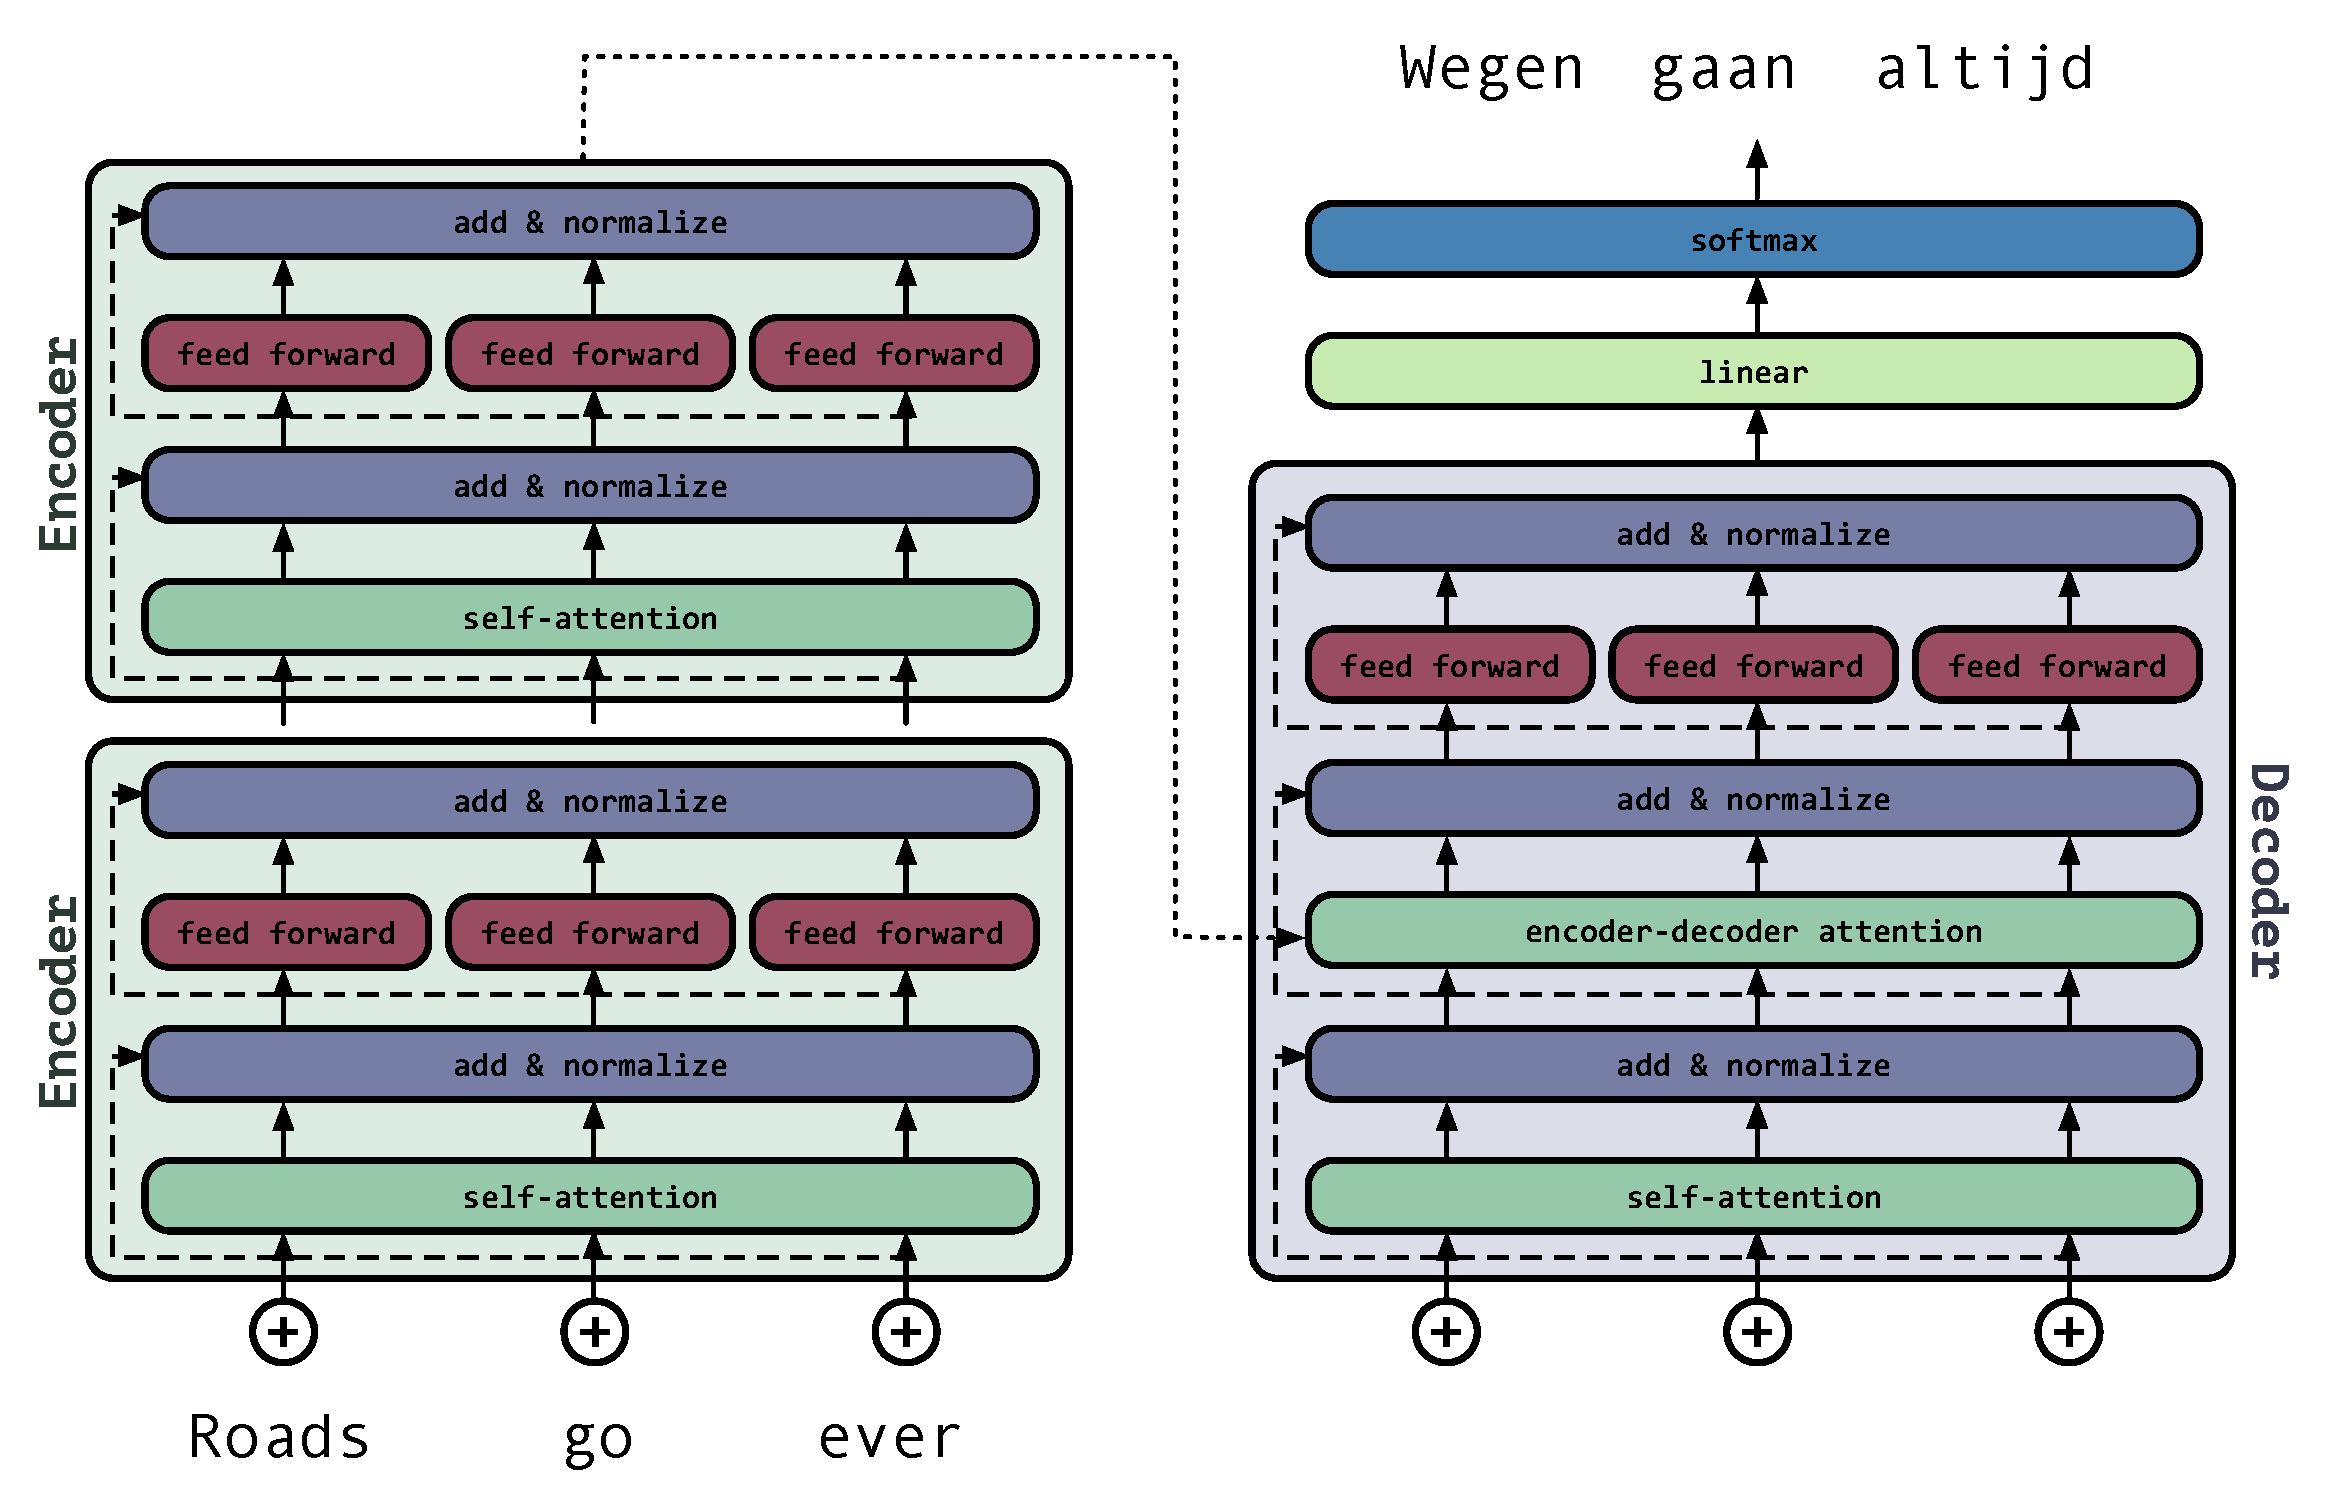
\includegraphics[width=0.95\linewidth]{02-background/figs/trnarc.pdf}
\caption{An illustration of a Transformer model introduced in \citet{vaswani2017attention}.}
\label{bgTRNfig}
\end{figure}

\begin{figure}
\centering
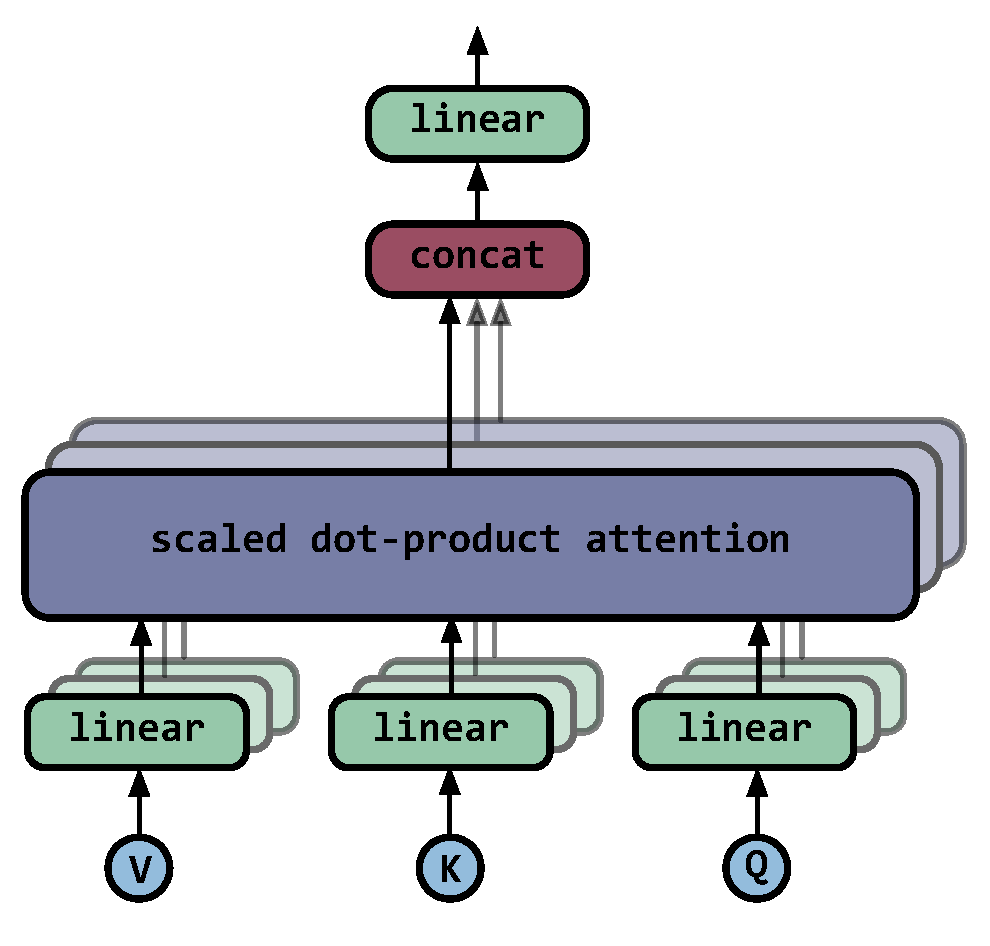
\includegraphics[width=0.5\linewidth]{02-background/figs/selfatt.pdf}
\caption{An illustration of self-attention in the Transformer model based on \citet{vaswani2017attention}.}
\label{bgTRNattfig}
\end{figure}


The transformer model is an encoder-decoder architecture without a sequential structure.
The encoder is given an input sequence of tokens $X = \big[ x_1, \ldots, x_n \big] $, and encodes it as a continuous representation $\vt{X} = \big[\vt{x}_1, \ldots, \vt{x}_n \big] $ based on the attention. 
The decoder then generates the output sequence $Y = \big[ y_1, \ldots, y_m \big] $ token by token, given the representation $\vt{X}$ and the previously generated token. 
Figure~\ref{bgTRNfig} illustrates this architecture which we will discuss in detail below. 

For every token $x_i$ in the input sequence, we first create a query $\vt{q}_i$, a key $\vt{k}_i$, and a value $\vt{v}_i$ vector.
Self-attention then uses \textit{scaled dot product attention} (last row in Table~\ref{backgroundattentions}) to compute the attention score of token $x_i$ against other words in the input sequence.
This attention has a scaling factor where $n$ is the dimension of the source hidden states.
To calculate representation $\vt{x}_i$, a softmax layer is then used to normalize the self-attention scores and multiplies it with $\vt{v}_i$.
In practice, the attention is computed on matrices of inputs ($\vt{Q}, \vt{K}, \vt{V}$) as follows:
\begin{align}
\attention (\vt{Q}, \vt{K}, \vt{V}) = \softmax (\frac{\vt{K}^\intercal \vt{Q} }{\sqrt{d_k}})\vt{V}
\end{align}

\noindent where $d_k$ is the embedding dimension of the key vectors which scales the dot product. The encoder is a stacking of identical layers each consisting of a \textit{multi-head self-attention} layer and a point-wise fully connected feed-forward network.
$\vt{Q}$, $\vt{K}$, and $\vt{V}$ matrices are split up into multiple heads and the multi-head attention mechanism computes the attention in parallel. 
Each token in the sequence goes through the encoder independently. 
During encoding, there are dependencies between the paths of different tokens in the self-attention layer, but the feed-forward layer of each token does not have any dependencies.
As a result words in the sequence can be processed in parallel. 
The independent attention outputs are then concatenated and linearly projected as follows: %transformed into expected dimensions.
\begin{align}
\text{Multi-Head Attention} (\vt{Q}, \vt{K}, \vt{V}) &= \concat (\text{head}_1, \ldots \text{head}_h) \vt{W}^o 
\end{align}
\noindent
where
\begin{align}
\text{head}_i = \attention(\vt{Q}\vt{W}_i^Q, \vt{K}\vt{W}_i^K, \vt{V}\vt{W}_i^V) 
\end{align}
\noindent
where $\vt{W}_i^Q, \vt{W}_i^K, \vt{W}_i^V$ are weight matrices that map the input representations to the query, key, and value matrices. $\vt{W}^o$ is the linear transformation that generates the output. 
All weight matrices are learned during training of the model.
Figure ~\ref{bgTRNattfig} illustrates this component. 
Similarly to the encoder, the decoder consists of a stack of identical layers, as well as a third sub-layer, which computes multi-head attention over the output of the encoder stack.
The self-attention layers in the decoder work slightly differently from the ones in the encoder. 
The computation of attention is \textit{masked} before the softmax step to prevent looking to the future of the sequence during training. 

Finally, there is a fully connected neural network that transforms the output of the stack of decoders into the target vocabulary vector.
The softmax function turns the scores into probabilities and the word with the highest probability is generated (greedy decoding). 
Alternatively, decoding can be done using the beam search technique similar to the RNN models discussed in Section~\ref{bgrnninference}.

\subsection{Residual connections} 

Another effective detail of the transformer architecture is the inclusion of residual connections \citep{He2016DeepRL} to facilitate optimization.
Residual connections connect the output of one layer with the input of an earlier layer.
Every self-attention and feed-forward neural network in the encoder and the decoder stack has a residual connection around it and a normalization layer \citep{Ba2016LayerN}.
This shortcut connection is particularly effective in training very deep architectures and mitigates the vanishing gradient problem. 

\subsection{Positional Encoding}

As discussed earlier, the transformer model does not have a recurrent structure and can be trained with a high degree of parallelization. 
However, languages are structured sequentially and it is necessary to encode some form of word order in the sequence \citep{tran-etal-2018-importance}. 
To address this shortcoming, the transformer adds a positional encoding vector to every word in the input sequence. 
These embeddings model the position of each word, or the relative distance between different words in the input.

\citet{vaswani2017attention} proposed sine and cosine functions of different frequencies to compute positional encodings:
\begin{align}
\text{positional encoding}_{(i, \delta)} = \begin{cases}
    \sin (\frac{i}{10000^{2\delta'/d}}) & \text{if $\delta = 2\delta'$}\\
        \\[5pt]
    \cos (\frac{i}{10000^{2\delta'/d}}) & \text{if $\delta = 2\delta' + 1$}
  \end{cases}
\end{align}

\noindent where $i$ is the position and $\delta = 1, \ldots, d$ is the dimension.
They also experimented with learned positional embeddings similar to \citet{pmlr-v70-gehring17a}, by assigning each input token with a learned vector that encodes its absolute position, and observed similar results to the sinusoidal version. 

